\documentclass[12pt,a4paper]{article}
\usepackage[utf8]{inputenc}
\usepackage[T1]{fontenc}
\usepackage[spanish]{babel}
\usepackage[margin=2.5cm]{geometry}
\usepackage{graphicx}
\usepackage{booktabs}
\usepackage{tabularx}
\usepackage{longtable}
\usepackage{xcolor}
\usepackage[hidelinks]{hyperref}
\setlength{\emergencystretch}{3em}
\newcommand{\pendiente}[1]{\par\noindent\textcolor{red!65!black}{\textbf{Pendiente:} #1}\par}
\begin{document}
\begin{titlepage}
\centering

\textbf{\Large Universidad de Ingeniería y Tecnología}\par
\vspace{0.3cm}
\textbf{\large UTEC}\par
\vspace{0.7cm}

% Colocar el logo oficial con este nombre en la carpeta imagenes.
\IfFileExists{imagenes/utec_logo.png}{
  
\includegraphics[width=4cm,height=2cm,keepaspectratio]{imagenes/utec_logo.png}%
}
\par\vspace{0.6cm}

\textbf{\large Curso: CS2032 -- Cloud Computing}\par
\vspace{0.8cm}

\textbf{\LARGE Sistema de gestión aeroportuaria basado en microservicios en AWS}\par
\vspace{0.4cm}
\textit{\large Integración de servicios, frontend y analítica de datos}\par
\vspace{0.7cm}

\textbf{\large Proyecto Parcial -- Hito 2}\par
\vspace{0.7cm}

\textbf{Integrantes:}\par
\vspace{0.3cm}
\renewcommand{\arraystretch}{1.35}
\begin{tabularx}{\textwidth}{X c}
\toprule
\textbf{Estudiante} & \textbf{Código} \\
\midrule
Benjamín Toro Leddihn & 202510596 \\
Guillermo Heredia Cardenas & 202410219 \\
Mariano Sánchez Arce & 202410653 \\
Edinson Vasquez Mamani & 202510680\\
Fabricio Cruz Trejo & 202420083 \\
Alexander Leon Pantaleon & 202510035 \\
\bottomrule
\end{tabularx}

\vfill
\textbf{Profesor:} [nombre completo pendiente]\par
\vspace{0.4cm}
\textbf{Ciclo académico:} 2026--2\par
\vspace{0.3cm}
\textbf{Lima, Perú -- Setiembre 2026}

\end{titlepage}

\tableofcontents
\clearpage
\section{Introducción y objetivos}
\textit{Responsable: Benjamín.}

\pendiente{Contexto del Aeropuerto Internacional Jorge Chávez; objetivos, alcance y relación con la rúbrica.}

\subsection{Implementación y decisiones}
\pendiente{Redactar esta sección con el estado real del proyecto.}

\subsection{Resultados y evidencias}
\pendiente{Incluir las evidencias identificadas en la plantilla del informe y describir lo que demuestran.}

\clearpage
\section{Arquitectura de solución}
\textit{Responsable: Benjamín.}

\pendiente{Describir los servicios AWS realmente utilizados, las capas y los flujos de operación, persistencia e ingesta. Incorporar el diagrama de arquitectura y justificar las decisiones del Learner Lab.}

\subsection{Implementación y decisiones}
\pendiente{Redactar esta sección con el estado real del proyecto.}

\subsection{Resultados y evidencias}
\pendiente{Incluir las evidencias identificadas en la plantilla del informe y describir lo que demuestran.}

\clearpage
\section{Backend y modelos de datos}
\label{sec:backend}
\textit{Responsable: Guillermo, Mariano, Edinson y Fabricio.}

El backend está compuesto por cinco microservicios en Docker, con tres
lenguajes y tres motores de base de datos distintos, más dos servicios
sin persistencia propia:

\begin{table}[htbp]
\centering\small
\begin{tabularx}{\textwidth}{p{0.06\textwidth}p{0.24\textwidth}p{0.20\textwidth}p{0.14\textwidth}X}
\toprule
MS & Rol funcional & Lenguaje / framework & Motor & Puerto interno \\
\midrule
MS1 & Pasajeros / Tickets & Python + FastAPI & MySQL 8 & 8001 \\
MS2 & Vuelos / Operaciones & Java + Spring Boot & PostgreSQL 16 & 8002 \\
MS3 & Infraestructura / Incidencias & Node.js + Express & MongoDB 7 & 3003 \\
MS4 & Manifiesto de vuelo & Python + FastAPI & sin BD (agregador) & 8004 \\
MS5 & Analítico & Python + FastAPI + boto3 & sin BD (Athena) & 8005 \\
\bottomrule
\end{tabularx}
\caption{Los cinco microservicios: tres con base propia y dos sin
persistencia. Los tres primeros exponen sus datos operacionales; MS4
agrega vía HTTP; MS5 consulta el data lake.}
\label{tab:ms-backend}
\end{table}

\subsection{Implementación y decisiones}

\subsubsection{MS1 --- Pasajeros / Tickets (Guillermo)}
MS1 cubre el dominio de pasajeros del aeropuerto Jorge Chávez: categorías
migratorias, pasajeros, emisión de tickets, check-in y equipaje. Se
implementa en Python 3.12 con FastAPI 0.115, SQLAlchemy 2 como ORM, Alembic
para las migraciones versionadas y MySQL 8. La API corre en el puerto
interno 8001 bajo el prefijo público \texttt{/api/pasajeros} (nginx). La
URL de MS2 se configura por variable de entorno
(\texttt{MS2\_BASE\_URL}, cliente \texttt{httpx} con timeout de 3\,s y 2
reintentos), de modo que el mismo código consume el MS2 real en producción
o el mock local en desarrollo.

\begin{figure}[htbp]
  \centering
  \IfFileExists{imagenes/swagger-ms1.png}{%
    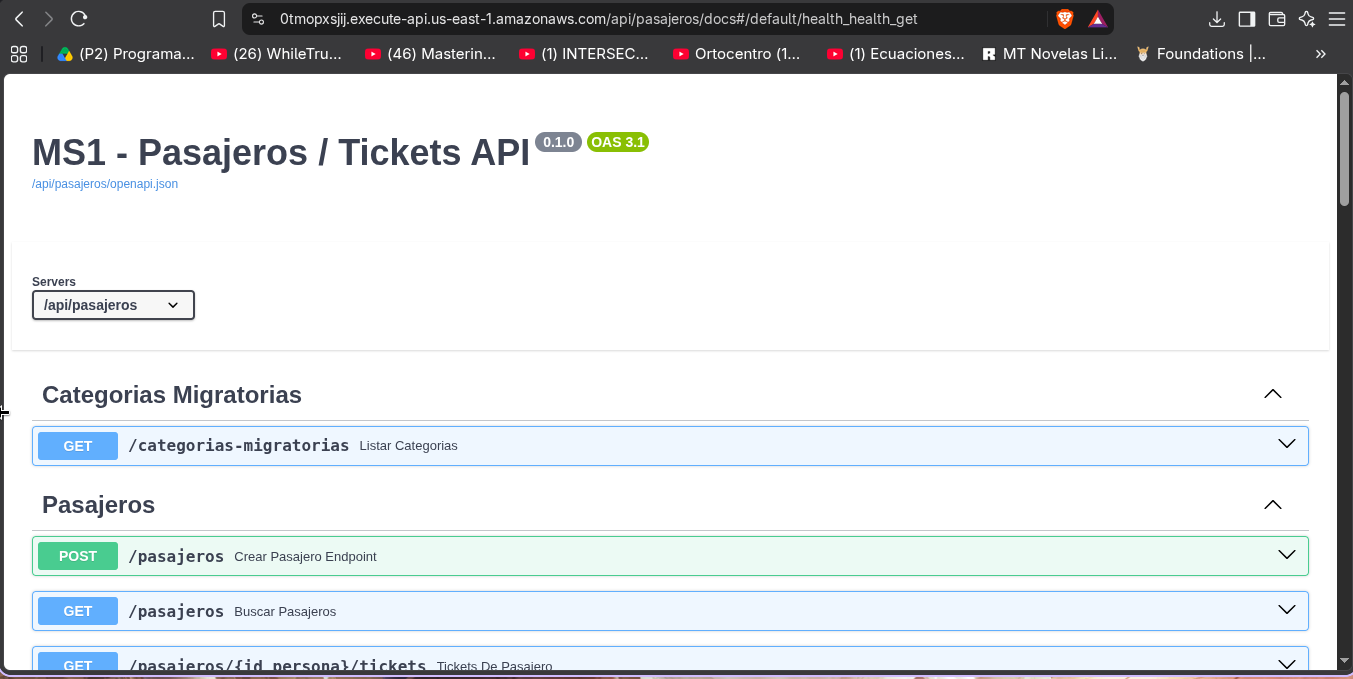
\includegraphics[width=0.95\linewidth]{imagenes/swagger-ms1.png}%
  }{%
    \fbox{\parbox{0.90\linewidth}{\centering\textbf{Swagger-UI de MS1}\par
    Copiar \texttt{swagger-ms1.png} a \texttt{imagenes/} y recompilar.}}%
  }
  \caption{Swagger-UI de MS1 (\texttt{/docs}). Evidencia E-3.1.1.}
  \label{fig:swagger-ms1}
\end{figure}

\paragraph{Modelo de datos.}
El esquema (una migración Alembic, revisión \texttt{6ca35b598ec2}) tiene
seis tablas sobre MySQL 8 con los enums canónicos de
\texttt{contratos/enums.md} (sin tildes, para que los \texttt{JOIN} de
Athena coincidan):

\begin{table}[htbp]
\centering\small
\begin{tabularx}{\textwidth}{p{0.20\textwidth}p{0.22\textwidth}p{0.34\textwidth}X}
\toprule
Tabla (PK) & Columnas & Relación \\
\midrule
\texttt{persona} (\texttt{id\_persona}) & \texttt{nombre},
\texttt{apellido}, \texttt{fecha\_nacimiento} & superclase de identidad \\
\texttt{categoria\_migratoria} (\texttt{id}) & \texttt{nombre} ENUM,
\texttt{tarifa} & \texttt{CHECK(tarifa >= 0)}; 1--N \texttt{pasajero}
(3 filas: Nacional 12.50, Internacional 38.45, Transito 18.00 PEN) \\
\texttt{pasajero} (\texttt{id\_persona}) & \texttt{tipo\_documento} ENUM,
\texttt{numero\_documento}, \texttt{id\_categoria} &
\texttt{UNIQUE(tipo\_documento, numero\_documento)}; 1:1 IsA con
\texttt{persona} \\
\texttt{ticket} (\texttt{id\_ticket}) & \texttt{precio},
\texttt{fecha\_emision}, \texttt{estado\_boarding} ENUM,
\texttt{id\_vuelo}, \texttt{id\_persona} & \texttt{id\_vuelo} soft
$\to$ MS2; rango 1--60\,000; 1--1 \texttt{checkin} \\
\texttt{checkin} (\texttt{id\_ticket}) & \texttt{fecha\_hora},
\texttt{counter}, \texttt{con\_equipaje} & entidad débil 1:1 con
\texttt{ON DELETE CASCADE} \\
\texttt{equipaje} (\texttt{id} Tag BHS) & \texttt{peso},
\texttt{id\_persona}, \texttt{id\_vuelo} & \texttt{CHECK(peso > 0)};
\texttt{id\_vuelo} soft $\to$ MS2 \\
\bottomrule
\end{tabularx}
\caption{Esquema MySQL de MS1 (6 tablas).}
\label{tab:ms1-db}
\end{table}

\texttt{ticket.id\_vuelo} y \texttt{equipaje.id\_vuelo} son
\textbf{referencias suaves} a MS2: no hay FK física y su integridad se
valida por REST al escribir (Sección~\ref{sec:transformaciones}). El
diagrama E/R de la base se muestra en la Figura~\ref{fig:er-ms1}.

\begin{figure}[htbp]
  \centering
  \IfFileExists{imagenes/ms1-mysql-er.png}{%
    \includegraphics[width=0.95\linewidth]{imagenes/ms1-mysql-er.png}%
  }{%
    \fbox{\parbox{0.90\linewidth}{\centering\textbf{E/R de MS1}\par
    Copiar \texttt{ms1-mysql-er.png} a \texttt{imagenes/} y recompilar.}}%
  }
  \caption{E/R de la base MySQL de MS1 (6 tablas). Evidencia E-3b.1.}
  \label{fig:er-ms1}
\end{figure}

\paragraph{Endpoints implementados.}
Bajo la base pública \texttt{/api/pasajeros}:

\begin{table}[htbp]
\centering\small
\begin{tabularx}{\textwidth}{p{0.06\textwidth}p{0.19\textwidth}p{0.50\textwidth}X}
\toprule
Método & Ruta & Descripción \\
\midrule
GET & \texttt{/health}, \texttt{/health/db} & Estado del servicio y de la conexión MySQL \\
GET & \texttt{/categorias-migratorias} & Las 3 categorías con tarifa TUUA \\
POST & \texttt{/pasajeros} & Crea \texttt{persona}+\texttt{pasajero}; 409 si documento duplicado \\
GET & \texttt{/pasajeros} & Lista con filtros \texttt{tipo\_documento} y \texttt{numero\_documento} \\
GET & \texttt{/pasajeros/\{id\}} & Pasajero por id; 404 si no existe \\
GET & \texttt{/pasajeros/\{id\}/tickets} & Tickets de un pasajero \\
POST & \texttt{/tickets} & Emite ticket; valida el vuelo contra MS2 \\
GET & \texttt{/tickets} & Lista con filtro \texttt{vuelo\_id} \\
GET & \texttt{/tickets/\{id\}} & Ticket por id; 404 si no existe \\
POST & \texttt{/tickets/\{id\}/checkin} & Check-in 1:1; segundo intento $\to$ 409 \\
POST & \texttt{/equipajes} & Registra equipaje (Tag BHS único); valida vuelo contra MS2 \\
GET & \texttt{/equipajes} & Lista con filtros \texttt{pasajero\_id} y \texttt{vuelo\_id} \\
\bottomrule
\end{tabularx}
\caption{Endpoints de MS1.}
\label{tab:ms1-endpoints}
\end{table}

Los errores siguen el contrato común: cuerpo
\texttt{\{"error": \{"code": ..., "message": ...\}\}} con los códigos 400
(validación), 404 (no encontrado), 409 (duplicado), 422 (precondición no
cumplida, e.\,-g.\ vuelo inexistente o cancelado) y 502 (MS2 no
disponible).

\paragraph{Consumo entre servicios (MS1$\to$MS2).}
Al emitir un ticket o registrar un equipaje, MS1 valida el vuelo con
\texttt{GET /api/vuelos/\{id\}/exists} de MS2. En la verificación real
contra producción (23-Set-2026), \texttt{POST /api/pasajeros/tickets} con
\texttt{\{"precio": 45.5, "fecha\_emision": "2026-09-23", "id\_vuelo": 1,
"id\_persona": 100003\}} respondió \texttt{201} y el log del contenedor
registró la llamada saliente \texttt{Saliente MS1$\to$MS2: GET
http://ms2:8002/api/vuelos/1/exists $\to$ 200}. El log completo está en
\texttt{docs/evidencias/backend/consumo-entre-microservicios-2026-09-23.txt}.

\paragraph{Carga masiva y volumen.}
La base se pobló con los CSVs compartidos de
\texttt{aeropuerto-data-science/seeds/} (generador de Dev D, \texttt{SEED}
fijo) mediante \texttt{app/scripts/load\_csv.py}, ejecutado contra la VM
de producción con inserciones por lotes vía SQLAlchemy. El
\texttt{COUNT(*)} real (23-Set-2026) fue: \texttt{persona} 60\,000,
\texttt{pasajero} 60\,000, \texttt{ticket} 25\,000, \texttt{equipaje}
22\,814 y \texttt{checkin} 16\,577, superando el mínimo de 20\,000 en
\texttt{ticket} y \texttt{equipaje}
(\texttt{docs/evidencias/backend/ms1-count-2026-09-23.txt}).

\paragraph{Pruebas.}
La API se acompaña de 32 pruebas \texttt{pytest} sobre una base SQLite
in-memory (sin MySQL) que cubren los happy paths de pasajero, ticket,
check-in y equipaje, y los errores del contrato (404/409/422/502),
incluida la validación MS1$\to$MS2 de vuelo inexistente y cancelado. Smoke
end-to-end completo y log MS1$\to$MS2 en \texttt{smoke\_test.txt} y
\texttt{log\_ms1\_ms2.txt} del repositorio.

\subsubsection{MS2 --- Vuelos / Operaciones (Mariano)}
MS2 es responsable del dominio operacional del aeropuerto: vuelos,
aerolíneas, aeronaves, asientos y la tripulación asignada a cada vuelo.
Se implementa en Java 21 con Spring Boot 4.0.8, persistencia con
Spring Data JPA sobre PostgreSQL 16, migraciones versionadas con
Flyway y documentación OpenAPI con springdoc.

\begin{figure}[htbp]
  \centering
  \IfFileExists{imagenes/swagger-ms2.png}{%
    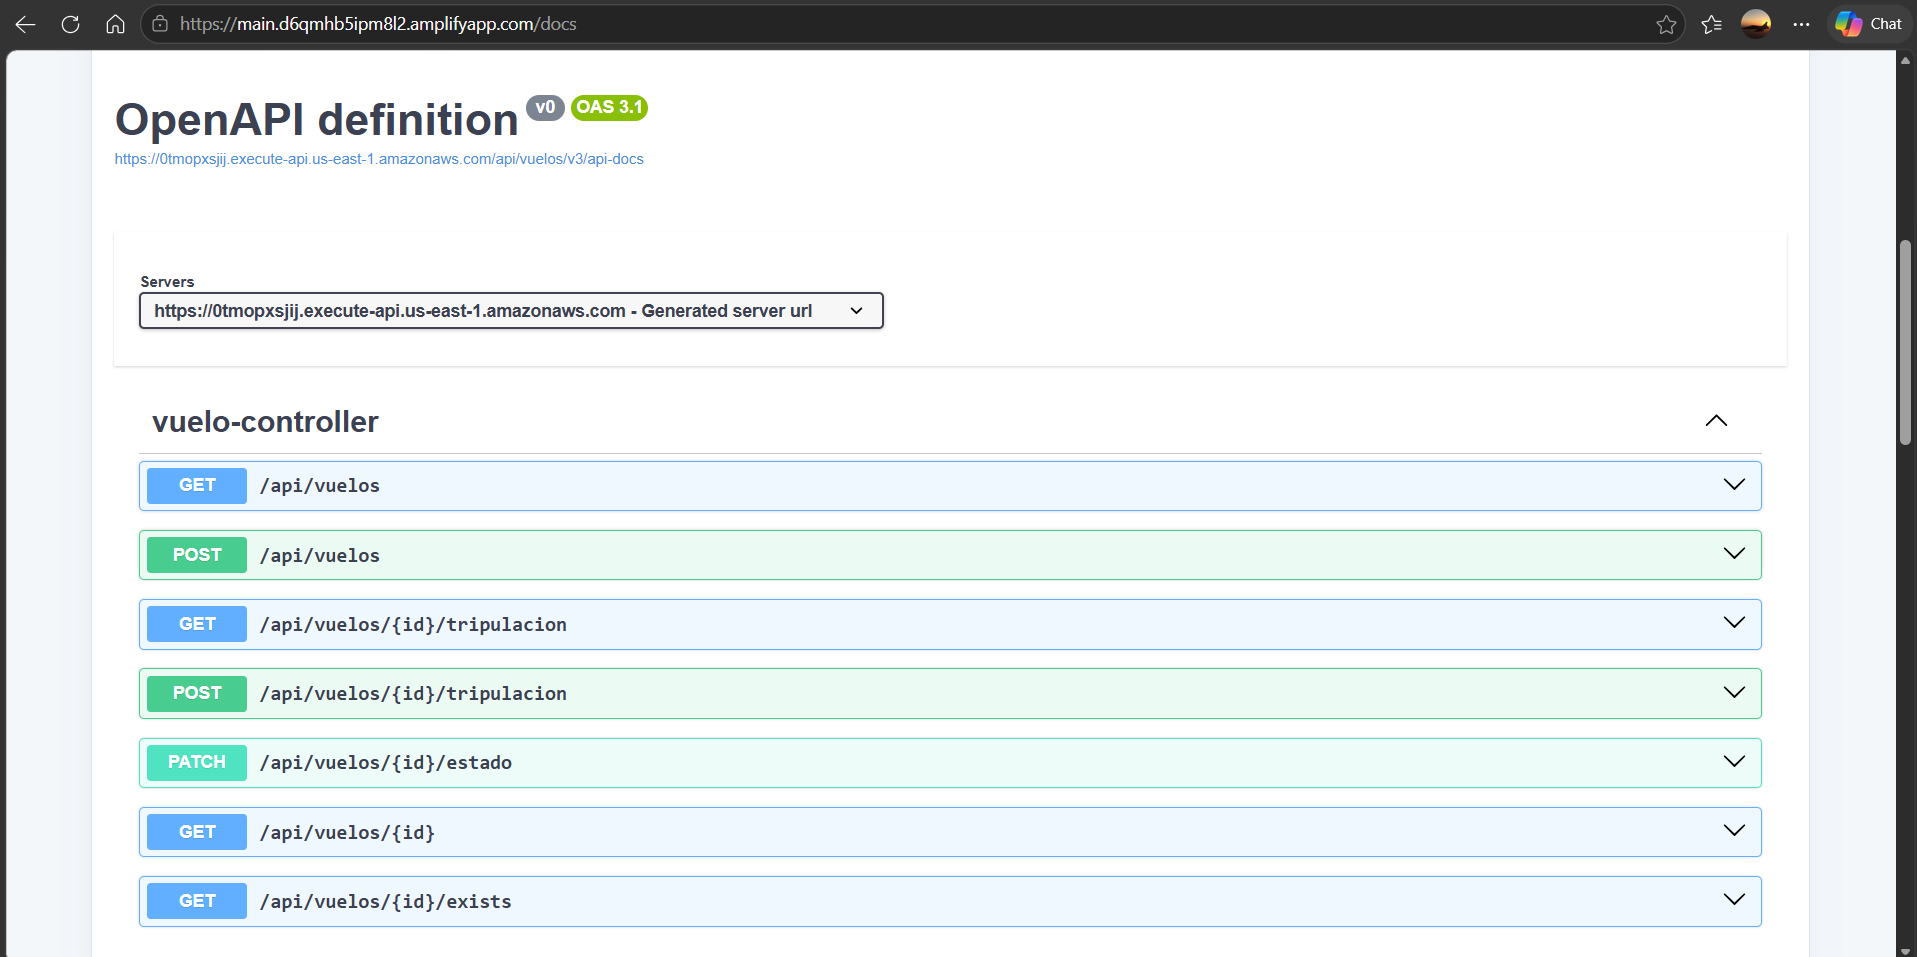
\includegraphics[width=0.95\linewidth]{imagenes/swagger-ms2.png}%
  }{%
    \fbox{\parbox{0.90\linewidth}{\centering\textbf{Swagger-UI de MS2}\par
    Copiar \texttt{swagger-ms2.png} a \texttt{imagenes/} y recompilar.}}%
  }
  \caption{Swagger-UI de MS2 (\texttt{/docs}) por la URL pública. Evidencia E-3.2.1.}
  \label{fig:swagger-ms2}
\end{figure}

El modelo de datos tiene ocho tablas: \texttt{aerolinea}, \texttt{aeronave},
\texttt{asiento}, \texttt{vuelo}, \texttt{empleado}, \texttt{tripulacion},
\texttt{operativo\_tierra} y \texttt{opera\_tripulacion}. Las relaciones
principales son \texttt{aerolinea} 1--N \texttt{vuelo}, \texttt{aeronave}
1--N \texttt{vuelo}, \texttt{aeronave} 1--N \texttt{asiento} (entidad
débil) y \texttt{tripulacion} N--M \texttt{vuelo} vía la tabla puente
\texttt{opera\_tripulacion}. Las claves naturales del modelo monolítico
se conservan: \texttt{aerolinea.ruc} y \texttt{aeronave.placa}, en vez
de identificadores autogenerados.

\texttt{empleado} reemplaza a la superclase \texttt{Persona} del modelo
original para el personal del aeropuerto (identidad propia del
servicio, ver Sección~\ref{sec:transformaciones}), con dos subtipos
modelados como patrón IsA de JPA (\texttt{@MapsId}): \texttt{tripulacion}
(\texttt{num\_licencia}) y \texttt{operativo\_tierra}
(\texttt{area\_operativa}), cada una con su propia primary key
compartida con \texttt{empleado.id}. La tabla puente
\texttt{opera\_tripulacion} usa una clave primaria compuesta
(\texttt{vuelo\_id}, \texttt{tripulacion\_empleado\_id}), modelada en
JPA con \texttt{@IdClass} sobre una clase auxiliar sin correspondencia
a ninguna tabla propia.

Los endpoints, bajo el prefijo \texttt{/api/vuelos}, cubren CRUD de
\texttt{aerolineas} (PK \texttt{ruc}) y \texttt{aeronaves} (PK
\texttt{placa}, con \texttt{GET /aeronaves/\{placa\}/asientos}), CRUD de
\texttt{vuelos} con filtros combinables \texttt{?num=\&estado=\&tipo=\&fecha=}
implementados con \texttt{JpaSpecificationExecutor} (construye la
consulta SQL dinámicamente según qué parámetros llegan, sin un método
por cada combinación), consulta de \texttt{empleados} por id o por
\texttt{tipo}, y asignación N--M de tripulación a un vuelo
(\texttt{POST}/\texttt{GET /vuelos/\{id\}/tripulacion}).

La Figura~\ref{fig:swagger-ms2} muestra el Swagger-UI navegable con los
15 endpoints implementados.

\texttt{PATCH /vuelos/\{id\}/estado} implementa una máquina de estados
explícita (\texttt{EstadoVueloMaquina}) sobre el enum
\texttt{estado\_vuelo}: \texttt{Programado} puede pasar a
\texttt{Embarcando}, \texttt{Retrasado} o \texttt{Cancelado};
\texttt{Embarcando} a \texttt{Despegado}, \texttt{Retrasado} o
\texttt{Cancelado}; \texttt{Retrasado} a \texttt{Embarcando},
\texttt{Despegado} o \texttt{Cancelado}; \texttt{Despegado} únicamente a
\texttt{Aterrizado}; \texttt{Aterrizado} y \texttt{Cancelado} son
estados finales sin transiciones salientes. Una transición fuera de esa
tabla responde \texttt{422 TRANSICION\_ESTADO\_INVALIDA}, siguiendo el
contrato de errores común. Al transicionar a \texttt{Despegado},
\texttt{hora\_real} se registra automáticamente con la hora del
servidor.

\texttt{GET /vuelos/\{id\}/exists} es el endpoint liviano de validación
consumido por MS1 (al emitir un ticket) y MS3 (al registrar una
incidencia o asignación que referencia un vuelo): responde
\texttt{200 \{exists, estado\}} si el vuelo existe y \texttt{404} en
caso contrario, evitando que los servicios consumidores traigan el
objeto completo solo para verificar existencia. Es el mismo mecanismo
de referencia suave descrito en la Sección~\ref{sec:transformaciones}.

El consumo real de este endpoint está verificado con logs de
producción: MS1 lo invoca al emitir un ticket
(\texttt{GET /api/vuelos/1/exists} $\to$ \texttt{200}, previo a un
\texttt{POST /tickets} exitoso) y MS3 lo invoca al validar un vuelo
inexistente, traduciendo la respuesta \texttt{404} de MS2 a
\texttt{502 DEPENDENCIA\_ERROR} en su propio contrato (ver
\texttt{docs/evidencias/backend/consumo-entre-microservicios-2026-09-23.txt}).

Como el rango de \texttt{vuelo.id} es fijo y compartido entre servicios
(1--25\,000, ver \texttt{contratos/enums.md}), el siguiente id se
calcula con \texttt{SELECT COALESCE(MAX(id), 0) + 1} vía \texttt{@Query}
en el repositorio, en vez de traer todas las filas a memoria. Es
suficiente para el alcance del proyecto (pruebas manuales, sin
escrituras concurrentes reales); se documenta como limitación conocida,
no como pendiente.

El manejo de errores sigue el contrato común mediante un
\texttt{@RestControllerAdvice} único (\texttt{GlobalExceptionHandler})
que traduce las excepciones de dominio a los códigos acordados:
\texttt{VALIDACION} (400), \texttt{NO\_ENCONTRADO} (404),
\texttt{CONFLICTO\_ESTADO} (409) y \texttt{TRANSICION\_ESTADO\_INVALIDA}
(422).

\textbf{Carga masiva.} El generador de datos ficticios
(\texttt{seed/generar\_seed.py}) usa \texttt{Faker} con \texttt{SEED}
fijo e inserciones por lote (\texttt{execute\_values} de psycopg2) para
poblar 5 aerolíneas, 100 aeronaves, 21\,000 asientos, 300 empleados de
tripulación, 20\,500 vuelos y sus asignaciones N--M de tripulación. Se
empaqueta como contenedor Docker independiente y se ejecuta una sola
vez contra la base de datos objetivo.

\subsubsection{MS3 --- Infraestructura / Incidencias (Edinson)}
MS3 gestiona la infraestructura aeroportuaria: el inventario de
\textbf{recursos} (mangas y radares), las \textbf{incidencias}
operativas y las \textbf{asignaciones} vuelo--recurso. Se implementa en
Node.js con Express 4 y Mongoose sobre MongoDB 7 (base
\texttt{infra\_db}). Escucha en el puerto 3003 en local (8003 en
producción, \texttt{ms2:8002} como \texttt{MS2\_URL}) bajo el prefijo
\texttt{/api/infra}, más \texttt{GET /health} para los \emph{health
checks} del compose de producción.

\paragraph{Modelo de datos.}
Tres colecciones validadas con \textbf{AJV} (JSON Schema) antes de
insertar; los esquemas viven en \texttt{src/schemas/} y se documentan en
\texttt{docs/er/ms3-mongo-schemas.md}:
\begin{itemize}
  \item \texttt{recursos}: \texttt{id} entero, \texttt{nombre\_tecnico\_locacion}
    y \texttt{tipo} (\texttt{manga} o \texttt{radar}), más un
    subdocumento específico del tipo: \texttt{manga} con
    \texttt{estado\_acople} (\texttt{Libre}, \texttt{Ocupado},
    \texttt{Mantenimiento}, \texttt{Inoperativa}), \texttt{longitud} y
    \texttt{clase\_max} (letra \texttt{A}--\texttt{F}); o \texttt{radar}
    con \texttt{rango\_alcance}, \texttt{frecuencia} (\texttt{Banda L},
    \texttt{Banda S}, \texttt{Banda C}, \texttt{Banda X}) y
    \texttt{estado\_radar}.
  \item \texttt{incidencias}: \texttt{id}, \texttt{gravedad}
    (\texttt{Leve}, \texttt{Moderada}, \texttt{Alta}, \texttt{Critica}),
    \texttt{descripcion}, \texttt{tipo\_incidencia}
    (\texttt{Falla\_Radar}, \texttt{Inundacion},
    \texttt{Falta\_Combustible}, \texttt{Saturacion\_Vial},
    \texttt{Manga\_Inoperativa}, \texttt{Otro}), \texttt{fecha\_reporte}
    y \texttt{fecha\_cierre} opcional (nulo mientras está abierta), más
    los arreglos \texttt{afecta\_recursos[]} (\texttt{recurso\_id}) y
    \texttt{retrasa\_vuelos[]} (\texttt{vuelo\_id}). Esta colección es
    la que el data lake aplana en tres archivos (Sección~\ref{sec:data-science}).
  \item \texttt{asignaciones}: \texttt{recurso\_id} y \texttt{vuelo\_id}
    obligatorios, \texttt{fecha\_inicio}/\texttt{fecha\_fin} opcionales
    y \texttt{estado\_asignacion} (\texttt{Programada}, \texttt{En\_Curso},
    \texttt{Finalizada}, \texttt{Cancelada}).
\end{itemize}
Las consultas por identificador usan \texttt{findOne(\{ id \})} sobre un
índice único \texttt{id\_1}: el esquema de negocio expone el
\texttt{id} de dominio en lugar del \texttt{\_id} generado por Mongo.

\paragraph{Endpoints implementados.}
\begin{itemize}
  \item \textbf{Recursos}: \texttt{GET /recursos} con filtros
    \texttt{?tipo=} y \texttt{?estado=}, \texttt{GET /recursos/\{id\}},
    \texttt{POST /recursos} y \texttt{PATCH /recursos/\{id\}/estado}
    (cambia \texttt{estado\_acople} en mangas o \texttt{estado\_radar}
    en radares).
  \item \textbf{Incidencias}: \texttt{GET /incidencias} con filtros
    \texttt{?tipo=}, \texttt{?desde=} y \texttt{?hasta=},
    \texttt{GET /incidencias/\{id\}}, \texttt{POST /incidencias} y
    \texttt{PATCH /incidencias/\{id\}/cierre}.
  \item \textbf{Asignaciones}: \texttt{GET /asignaciones} con
    \texttt{?vuelo\_id=} y \texttt{?recurso\_id=} y
    \texttt{POST /asignaciones}.
\end{itemize}

\paragraph{Consumo de MS2 y reglas de negocio.}
Al crear una incidencia, cada \texttt{vuelo\_id} de
\texttt{retrasa\_vuelos[]} se valida con
\texttt{GET /api/vuelos/\{id\}/exists} de MS2 (MS3$\to$MS2). El cliente
\texttt{ms2Client} usa \texttt{fetch} nativo con timeout de 3\,s y
traduce la respuesta de MS2 así: \texttt{404} del MS2 (vuelo inexistente)
$\to$ \texttt{502 DEPENDENCIA\_ERROR}; vuelo existente pero
\texttt{Cancelado} $\to$ \texttt{422 VUELO\_NO\_EXISTE}; MS2 caído o sin
respuesta $\to$ \texttt{502 DEPENDENCIA\_ERROR} o
\texttt{503 DEPENDENCIA\_TIMEOUT}. \texttt{POST /asignaciones} repite esa
validación y añade dos reglas: el recurso debe estar \texttt{Libre}
(solo aplica a mangas; si no, \texttt{409 RECURSO\_OCUPADO}), y
\texttt{clase\_max} de la manga debe ser mayor o igual que la clase de
la aeronave del vuelo, obtenida de \texttt{GET /api/vuelos/aeronaves/...}
de MS2 (\texttt{422 ACOPLE\_CLASE\_INVALIDO}). El cierre de incidencias
(\texttt{PATCH /incidencias/\{id\}/cierre}) fija \texttt{fecha\_cierre}
y rechaza un segundo cierre con \texttt{409 INCIDENCIA\_YA\_CERRADA}.
Los errores siguen el contrato común (\texttt{docs/contratos/errores.md})
con el formato \texttt{\{ error: \{ code, message, status, details,
service, timestamp \} \}}.

El consumo real quedó verificado contra producción el 23-Set-2026:
\texttt{POST /api/infra/incidencias} con
\texttt{retrasa\_vuelos=[\{vuelo\_id: 999999\}]} provocó la llamada
saliente \texttt{[MS3$\to$MS2] GET http://ms2:8002/api/vuelos/999999/exists}
en el log del contenedor, y MS3 tradujo el \texttt{404} de MS2 a
\texttt{502 DEPENDENCIA\_ERROR}
(\texttt{docs/evidencias/infra/ms3-consume-ms2-2026-09-23.txt}),
confirmando que la integración no es un mock.

\paragraph{Carga masiva y volumen.}
El generador compartido del \emph{data squad} (misma semilla, orden
MS2$\to$MS1$\to$MS3) emitió \textbf{500 recursos}, \textbf{25\,000
incidencias} y \textbf{40\,000 asignaciones}, con \texttt{vuelo\_id} en
el rango 1--25\,000 de MS2 para que los \emph{joins} del data lake no
queden vacíos. Se cargaron una única vez con \texttt{mongoimport} contra
la base \texttt{infra} en la VM-DB; la evidencia es
\texttt{db.incidencias.countDocuments()} = 25\,000 ($\geq$ 20\,000
exigidos) verificado con \texttt{mongosh} el 23-Set-2026
(\texttt{docs/evidencias/backend/ms3-count-2026-09-23.txt}).
La \texttt{ingesta-ms3} (DS-08) se ejecutó contra la BD real y subió a
\texttt{s3://mla-aeropuerto-lake/raw/ms3/} cinco archivos planos:
\texttt{recurso} (500), \texttt{incidencia} (25\,000),
\texttt{incidencia\_afecta\_recurso} (50\,136),
\texttt{incidencia\_retrasa\_vuelo} (46\,678) y \texttt{asignacion}
(40\,000).

\pendiente{Swagger-UI de MS3 (\texttt{swagger-ui-express}) no está
implementado en el código (falta la dependencia y la ruta
\texttt{/api/infra/docs}), por lo que el bullet compartido que afirma
que los cinco microservicios exponen \texttt{/docs} es falso para MS3.
Pendiente: agregar \texttt{swagger-ui-express}, publicar la imagen y
adjuntar la captura como Evidencia E-3.3.1 (MS3-09).}

\subsubsection{MS4 --- Manifiesto de vuelo (Fabricio)}
MS4 es un agregador HTTP sin base de datos propia. Recibe una petición
por un identificador de vuelo y compone una respuesta que consolida
información de MS1, MS2 y MS3, sin persistir nada. Se implementa en
Python con FastAPI 0.115 y \texttt{httpx.AsyncClient}.

Endpoints principales bajo el prefijo \texttt{/api/manifiesto}:

\begin{itemize}
  \item \texttt{GET /\{vuelo\_id\}}: manifiesto consolidado. Verifica
    primero que el vuelo exista consultando
    \texttt{GET /api/vuelos/\{id\}/exists} en MS2 (devuelve
    \texttt{404} sin gastar el resto de llamadas si el vuelo no existe).
    Luego lanza en paralelo con \texttt{asyncio.gather} cuatro
    peticiones: al vuelo completo con aeronave y aerolínea en MS2, a los
    tickets del vuelo con pasajeros y equipaje en MS1, a la tripulación
    en MS2 y a las incidencias abiertas del vuelo en MS3.
  \item \texttt{GET /\{vuelo\_id\}/pasajeros} y
    \texttt{/\{vuelo\_id\}/resumen}: subrecursos que reutilizan la misma
    infraestructura. El resumen calcula conteos: pasajeros totales,
    kilogramos de equipaje y número de incidencias abiertas.
  \item \texttt{GET /health/dependencias}: consulta en paralelo el
    \texttt{/health} de MS1, MS2 y MS3 y responde con un estado global
    (\texttt{up}, \texttt{degraded} o \texttt{down}).
\end{itemize}

El cliente HTTP compartido (\texttt{app/clients/base.py}) implementa
\emph{timeouts} de 3 segundos, reintentos exponenciales solo en errores
transitorios (\emph{timeout}, \texttt{ConnectError}, HTTP \texttt{5xx})
y propagación tal cual de errores \texttt{4xx}. Sirve como referencia
para el cliente que MS1 y MS3 usan al consumir MS2.

La estrategia de tolerancia a fallos (MS4-04) es clave: si alguna
dependencia responde con error o excede el timeout, MS4 no falla la
petición completa; el campo correspondiente queda vacío en la respuesta
y se agrega un mensaje al arreglo \texttt{warnings[]}. Un manifiesto
parcial es siempre preferible a un \texttt{500}. Esta decisión permite
que el frontend siga renderizando información útil aunque MS3 esté
inaccesible.

\subsubsection{MS5 --- Analítico sobre Athena (Fabricio)}
MS5 tampoco tiene base de datos propia: consulta el catálogo Glue
\texttt{aeropuerto\_lake} mediante \texttt{boto3}. Su
\texttt{AthenaClient} ejecuta cada consulta con
\texttt{start\_query\_execution}, hace \emph{poll} cada 500 ms a
\texttt{get\_query\_execution} hasta un estado terminal
(\texttt{SUCCEEDED}, \texttt{FAILED} o \texttt{CANCELLED}) con timeout
de 60 segundos, y luego pagina \texttt{get\_query\_results}
convirtiendo los valores a tipos Python (\texttt{bigint}$\to$\texttt{int},
\texttt{decimal}$\to$\texttt{float}, \texttt{NULL}$\to$\texttt{None}).
Un cache local por SHA-256 del SQL evita ejecuciones repetidas dentro
de \texttt{ATHENA\_CACHE\_TTL\_SECONDS} (300 s por defecto).

Los cinco endpoints exponen las consultas Q1--Q5 descritas en la
Sección \ref{sec:data-science}:

\begin{itemize}
  \item \texttt{/api/analitica/recursos-mas-fallas?dias=N}
  \item \texttt{/api/analitica/retraso-promedio?tipo=Nacional|Internacional}
  \item \texttt{/api/analitica/incidencias-combustible-por-aerolinea}
  \item \texttt{/api/analitica/recaudacion-tuua-por-categoria}
    (lee la vista \texttt{vw\_recaudacion\_tuua})
  \item \texttt{/api/analitica/vuelos-hora-punta-retrasados}
    (lee la vista \texttt{vw\_retrasos\_hora\_punta})
\end{itemize}

Los parámetros se validan con Pydantic (\texttt{Literal} para
\texttt{tipo}, \texttt{Query(ge=1, le=365)} para \texttt{dias}) antes de
interpolarse en el SQL: no hay riesgo de inyección. Los errores de
Athena se envuelven en \texttt{AthenaQueryError} y se mapean a HTTP
\texttt{502} siguiendo el contrato común de errores
(\texttt{ATHENA\_QUERY\_ERROR}). En EC2 con Learner Lab, \texttt{boto3}
toma las credenciales del \texttt{LabInstanceProfile} automáticamente;
no se pasan claves en \texttt{.env}.

\subsubsection{Contratos y clientes compartidos}
Los cinco microservicios respetan los mismos contratos: el conjunto de
enums (\texttt{docs/contratos/enums.md}), los rangos de identificadores
(\texttt{docs/plan-de-trabajo.md \S3}) y el formato de errores
(\texttt{docs/contratos/errores.md}). El cliente HTTP con reintentos y
propagación de \texttt{X-Request-Id} de MS4 se reutiliza en MS1 y MS3
para las llamadas a MS2.

\subsection{Resultados y evidencias}

\begin{itemize}
  \item Los cinco servicios responden \texttt{/health} y exponen su
    especificación en \texttt{/openapi.json} y Swagger-UI en
    \texttt{/docs}. Los cinco \texttt{openapi.yaml} borrador viven en la
    raíz de cada repositorio.
  \item MS1 supera el mínimo de 20\,000 registros en sus dos tablas de
    volumen: \texttt{ticket} (25\,000) y \texttt{equipaje} (22\,814),
    verificado con \texttt{COUNT(*)} contra la VM-DB de producción el
    23-Set-2026 (\texttt{docs/evidencias/backend/ms1-count-2026-09-23.txt}),
    y consume a MS2 de forma verificada
    (\texttt{docs/evidencias/backend/consumo-entre-microservicios-2026-09-23.txt}).
  \item MS2 supera el mínimo de 20\,000 registros en sus dos tablas de
    volumen: \texttt{vuelo} (20\,500) y \texttt{asiento} (21\,000),
    verificado con \texttt{COUNT(*)} contra la VM-DB de producción el
    23-Set-2026 (\texttt{docs/evidencias/backend/ms2-count-2026-09-23.txt}).
  \item MS2 se acompaña de pruebas con \texttt{@SpringBootTest} y
    \texttt{MockMvc} que cubren el happy path de creación de aerolínea,
    validación de datos inválidos (\texttt{400 VALIDACION}), búsqueda
    de recursos inexistentes (\texttt{404 NO\_ENCONTRADO}),
    \texttt{GET /vuelos/\{id\}/exists} con y sin vuelo existente, y la
    lógica de la máquina de estados en aislamiento (unit test puro,
    sin base de datos, sobre \texttt{EstadoVueloMaquina}).
  \item MS4 se probó \emph{end-to-end} contra los MS1/MS2/MS3 reales
    durante el Hito 1: para el vuelo \texttt{id=1} devolvió el vuelo
    \texttt{CM0001 (Copa Airlines, LIM-TRU)}, la tripulación con
    licencias \texttt{DGAC-*} y una lista de incidencias, con
    \texttt{warnings[]} vacío cuando las tres dependencias respondieron.
    Al detener MS3, la misma petición devolvió \texttt{200} con
    \texttt{incidencias\_abiertas: []} y el warning correspondiente
    (evidencia de MS4-04).
  \item MS5 se acompaña de dieciséis pruebas unitarias con
    \texttt{MagicMock} del cliente \texttt{boto3.client("athena")} que
    cubren: éxito con conversión de tipos, \texttt{FAILED} $\to$
    \texttt{AthenaQueryError}, cache TTL, cache que no cruza entre
    consultas distintas, \texttt{NULL} $\to$ \texttt{None}, cada uno de
    los cinco endpoints con \texttt{200} y con \texttt{502}, y
    validación de parámetros fuera de rango con \texttt{422}. Todas
    pasan localmente sin necesidad de credenciales AWS.
  \item Imágenes de MS4 y MS5 publicadas en \texttt{v1.0} tras
    \texttt{git tag} + \texttt{git push --tags} (workflow
    \texttt{build-push-*} de cada repositorio). En \texttt{compose/vm-prod/}
    del repositorio de infraestructura se hace \texttt{docker compose
    pull \&\& up} para desplegar la última versión sin cambios de
    código.
\end{itemize}

\pendiente{Adjuntar el JSON completo del manifiesto y el JSON de una
consulta analítica ejecutada contra la infraestructura desplegada.}

\clearpage
\section{Transformaciones del modelo monolítico}
\label{sec:transformaciones}
\textit{Responsable: Fabricio.}

El modelo relacional único del proyecto de Base de Datos I se reparte en
tres sistemas de persistencia autónomos (MySQL, PostgreSQL y MongoDB), uno
por microservicio con base de datos. Ninguna tabla se comparte entre
motores. Las relaciones que en el monolito eran claves foráneas físicas se
transforman en \emph{referencias suaves} validadas por REST en tiempo de
escritura. Los enumerados que antes vivían como tipos \texttt{ENUM} en un
solo esquema se replican por servicio, sincronizados por
\texttt{docs/contratos/enums.md} para que los \texttt{JOIN} de Athena
funcionen.

\subsection{Implementación y decisiones}

\subsubsection{Descomposición por microservicio}
Las veintiuna relaciones del modelo original se distribuyen así:

\begin{itemize}
  \item \textbf{MS1 (MySQL)}: \texttt{persona}, \texttt{pasajero},
    \texttt{categoria\_migratoria}, \texttt{ticket}, \texttt{checkin},
    \texttt{equipaje}. Dueño de la identidad de los viajeros y de las
    transacciones comerciales.
  \item \textbf{MS2 (PostgreSQL)}: \texttt{vuelo}, \texttt{aerolinea},
    \texttt{aeronave}, \texttt{asiento}, \texttt{empleado},
    \texttt{tripulacion}, \texttt{operativo\_tierra},
    \texttt{opera\_tripulacion}. Dueño de la operativa aeroportuaria.
  \item \textbf{MS3 (MongoDB)}: colecciones \texttt{recursos},
    \texttt{incidencias} y \texttt{asignaciones}. Dueño de la
    infraestructura física del terminal y de la gestión de incidencias.
\end{itemize}

\subsubsection{Jerarquía \texttt{Persona} partida}
En el modelo E-R original, \texttt{Persona} es superclase de
\texttt{Pasajero} y también de \texttt{Personal} (a su vez superclase de
\texttt{Tripulacion} y \texttt{Operativo\_Tierra}). En una arquitectura de
microservicios no es viable compartir la tabla \texttt{persona} entre MS1
y MS2, pues cada servicio administra su propio motor. La transformación
adoptada es:

\begin{itemize}
  \item \textbf{MS1} conserva \texttt{persona} $\to$ \texttt{pasajero}
    (Class Table Inheritance). \texttt{Pasajero} tiene su propio
    \texttt{id\_persona} heredado y su clave alternativa por
    \texttt{(tipo\_documento, numero\_documento)}.
  \item \textbf{MS2} crea una tabla \texttt{empleado} con
    \texttt{nombre}, \texttt{apellido} y \texttt{fecha\_nacimiento}
    embebidos (equivalente a lo que Persona aportaba en el monolito), y
    sus dos subclases \texttt{tripulacion} (con \texttt{num\_licencia}) y
    \texttt{operativo\_tierra} (con \texttt{area\_operativa}). No hay
    tabla \texttt{persona} en MS2; los atributos de identidad se duplican
    de forma deliberada.
\end{itemize}

Esta duplicación es consciente y se acepta como el costo de la autonomía
por servicio. Los diagramas E-R publicados en \texttt{docs/er/} de cada
repositorio reflejan la duplicación.

\subsubsection{Referencias suaves entre servicios}
Los identificadores que en el monolito eran claves foráneas entre tablas
de distintos dominios se convierten en referencias validadas por REST:

\begin{itemize}
  \item \texttt{ms1.ticket.vuelo\_id} y \texttt{ms1.equipaje.vuelo\_id}
    apuntan a \texttt{ms2.vuelo.id}. En cada \texttt{POST /tickets} y
    \texttt{POST /equipajes}, MS1 llama a
    \texttt{GET /api/vuelos/\{id\}/exists} en MS2. Si el vuelo no existe
    o está \texttt{Cancelado}, MS1 responde \texttt{422} sin persistir.
  \item \texttt{ms3.incidencia.retrasa\_vuelos[].vuelo\_id} y
    \texttt{ms3.asignacion.vuelo\_id} apuntan a \texttt{ms2.vuelo.id}.
    MS3 valida los identificadores contra MS2 al crear la incidencia o
    la asignación.
  \item MS4 no persiste: agrega vía HTTP las respuestas de MS1, MS2 y
    MS3 al servir el manifiesto. Es el consumidor de todas las
    referencias suaves, no las valida ni las crea.
\end{itemize}

Los logs de los servicios registran cada llamada saliente
(\texttt{X-Request-Id} propagado por nginx), lo que constituye la
evidencia obligatoria de que un microservicio consume a otro.

\subsubsection{Enumerados replicados y contrato compartido}
El enunciado exige valores idénticos de enums entre los tres servicios
para que las agregaciones de Athena funcionen. Se centralizan en
\texttt{docs/contratos/enums.md} del repositorio de documentación:
\texttt{estado\_vuelo}, \texttt{tipo\_vuelo}, \texttt{tipo\_documento},
\texttt{alianza}, \texttt{estado\_boarding}, \texttt{estado\_acople},
\texttt{gravedad}, \texttt{tipo\_incidencia}, \texttt{tipo\_recurso},
\texttt{nombre\_categoria\_migratoria}, \texttt{area\_operativa},
\texttt{clase\_aeronave} (OACI) y \texttt{frecuencia\_radar}. Cada servicio
los implementa con la sintaxis nativa de su motor (PostgreSQL
\texttt{CREATE TYPE ... AS ENUM}, MySQL \texttt{ENUM} o \texttt{CHECK},
validación en la capa aplicativa de MongoDB), pero los \emph{strings}
coinciden byte a byte para que Athena pueda hacer \texttt{GROUP BY} y
\texttt{JOIN} sobre esas columnas sin normalizaciones intermedias. Los
valores no llevan tildes en enums (\texttt{Critica}, \texttt{Transito},
\texttt{Inundacion}) para evitar problemas de codificación en la ruta
CSV $\to$ Glue $\to$ Athena.

\subsubsection{Rangos de identificadores deterministas}
Para que los \texttt{JOIN} entre tablas de tres motores distintos
funcionen en Athena, los identificadores deben cruzarse aunque la
generación de datos ocurra en tres corridas independientes por servicio.
Se acuerdan en \texttt{docs/plan-de-trabajo.md \S3} rangos disjuntos por
entidad (\texttt{vuelo.id} 1--25\,000, \texttt{persona.id} 100\,000--160\,000,
\texttt{ticket.id} 1--60\,000, \texttt{recurso.id} 1--500,
\texttt{incidencia.id} 1--30\,000) y un \texttt{SEED} fijo
(\texttt{20\,260\,905}) para el generador \texttt{seeds/} compartido. El
orden interno del generador es \textbf{MS2 $\to$ MS1 $\to$ MS3} para que
los identificadores de vuelo existan antes de que se creen los tickets y
las incidencias que los referencian. Detalles en la Sección
\ref{sec:data-science}.

\subsection{Resultados y evidencias}

Las transformaciones descritas se materializan en artefactos verificables:

\begin{itemize}
  \item Los tres diagramas E-R por servicio residen en \texttt{docs/er/}
    del repositorio de documentación. Cada uno refleja únicamente las
    tablas de su motor, con la duplicación deliberada de atributos de
    identidad.
  \item Los archivos de contrato compartido: \texttt{docs/contratos/enums.md}
    (enumerados) y \texttt{docs/plan-de-trabajo.md \S3} (rangos de ID).
  \item Los generadores en \texttt{aeropuerto-data-science/seeds/}
    respetan los rangos y el orden acordado, y producen salida
    reproducible byte a byte con el mismo \texttt{SEED} (comprobado por
    igualdad de sumas MD5 entre corridas).
  \item La validación cruzada de las referencias suaves se ejecuta con
    las cinco consultas Q1--Q5 sobre Postgres local (Sección
    \ref{sec:data-science}); si un identificador no cruzara, los
    \texttt{JOIN} devolverían cero filas. Los resultados no vacíos
    confirman la integridad.
\end{itemize}

\clearpage
\section{Frontend}
\textit{Responsable: Alexander.}

\pendiente{Describir las cuatro vistas, integración con MS1 a MS5, estados de carga, error y vacío, responsive y Swagger agregado. Completar la matriz REST con verbo, ruta, servicio y evidencia. Confirmar con el equipo el criterio de métodos REST para MS4 y MS5, cuyas rutas son GET. Añadir la URL pública y capturas de integración real.}

\subsection{Implementación y decisiones}
\pendiente{Redactar esta sección con el estado real del proyecto.}

\subsection{Resultados y evidencias}
\pendiente{Incluir las evidencias identificadas en la plantilla del informe y describir lo que demuestran.}

\clearpage
\section{Data Science y catálogo de datos}
\textit{Responsable: Fabricio; Alexander para el diagrama del catálogo.}

\pendiente{Documentar S3, las tres ingestas, catálogo Glue, consultas Athena y dos vistas. Incorporar el diagrama E/R del catálogo y comprobar su correspondencia con el catálogo desplegado.}

\subsection{Implementación y decisiones}
\pendiente{Redactar esta sección con el estado real del proyecto.}

\subsection{Resultados y evidencias}
\pendiente{Incluir las evidencias identificadas en la plantilla del informe y describir lo que demuestran.}

\clearpage
\section{Despliegue y seguridad}
\textit{Responsable: Benjamín.}

Los 5 microservicios corren en \textbf{dos instancias EC2 idénticas} (VM-PROD-1, VM-PROD-2, subredes
privadas \texttt{10.0.0.10/24} y \texttt{10.0.1.0/24}), cada una con \texttt{docker compose} levantando
\texttt{nginx} + \texttt{ms1..ms5}. Un \textbf{Application Load Balancer interno} (\texttt{aeropuerto-alb},
\texttt{scheme=internal}) balancea el tráfico HTTP:80 entre ambas VM, con \textit{health check} sobre
\texttt{/api/pasajeros/health}. La única entrada pública es \textbf{Amazon API Gateway} (HTTP API), que
cruza un \textbf{VPC Link} hacia el ALB — API Gateway, ALB y VM-PROD se prueban de punta a punta con
\texttt{curl} real a la URL pública, sin mocks.

\subsection{Implementación y decisiones}

\textbf{Grupos de seguridad.} \texttt{sg-vm-prod} solo permite entrada TCP:80 desde \texttt{sg-alb}
(ningún puerto abierto a \texttt{0.0.0.0/0}); \texttt{sg-alb} solo desde \texttt{sg-apigw-vpclink};
\texttt{sg-vm-db} solo TCP 3306/5432/27017 desde \texttt{sg-vm-prod} y \texttt{sg-vm-ingesta}. Esta
configuración se abrió temporalmente el 21-Set-2026 (\texttt{0.0.0.0/0} en \texttt{sg-vm-prod}) para
poder probar directo mientras el registro de imágenes estaba roto, y se cerró el 22-Set-2026 una vez
publicadas las imágenes en Docker Hub — sin recrear las instancias, solo actualizando la regla del
Security Group (\texttt{terraform apply} con 0 recursos destruidos).

\textbf{Healthchecks.} Los 6 contenedores de cada VM-PROD (\texttt{nginx}, \texttt{ms1..ms5}) tienen
\texttt{healthcheck} activo en \texttt{docker-compose.yml}. Dos detalles no evidentes que costó
diagnosticar: (1) el healthcheck de \texttt{nginx} debe apuntar a \texttt{127.0.0.1}, no a
\texttt{localhost} — \texttt{wget} (busybox) resuelve \texttt{localhost} a \texttt{::1} primero y
\texttt{nginx} no escucha en IPv6, lo que daba \texttt{Connection refused} aunque el servidor
funcionara perfectamente; (2) el healthcheck de \texttt{ms1} debe apuntar a \texttt{/health} sin
prefijo, porque \texttt{nginx} sí recorta \texttt{/api/pasajeros/} para ese servicio en particular
(\texttt{proxy\_pass} con \texttt{"/"} final), a diferencia de \texttt{ms2..ms5} que reciben la URL
completa.

\textbf{Respaldo y reinicio.} \texttt{RUNBOOK.md} documenta la provisión inicial, el reinicio tras un
corte de sesión del Learner Lab (objetivo \textless{}15\,min) y la limpieza. El respaldo de las 3 bases
de datos se formalizó en \texttt{scripts/backup-db.sh}: sube un script autocontenido a S3 y lo ejecuta
en VM-DB por SSM Run Command (sin sesión interactiva), volcando MySQL, PostgreSQL y MongoDB a
\texttt{s3://mla-aeropuerto-lake/backups/}.

\subsection{Resultados y evidencias}

Corrida real del 22-Set-2026 (\texttt{docs/evidencias/infra/smoke-e2e-2026-09-22.txt}):

\begin{itemize}
\item \texttt{curl https://\{api-id\}.execute-api.us-east-1.amazonaws.com/api/pasajeros/health} $\to$
  \textbf{200 OK}, desde fuera de la VPC.
\item Acceso directo a las IP públicas de ambas VM-PROD: \textbf{timeout} (bloqueado por
  \texttt{sg-vm-prod}).
\item \texttt{nc -zv} al DNS del ALB interno desde fuera: \textbf{connection refused} — no es
  alcanzable públicamente, como corresponde a un ALB \texttt{internal}.
\item VM-DB y VM-INGESTA: sin IP pública (confirmado con \texttt{aws ec2 describe-instances}).
\item \texttt{docker compose ps} en ambas VM-PROD: los 6 servicios en estado \texttt{healthy}
  (\texttt{docs/evidencias/infra/docker-compose-ps-2026-09-22.txt}).
\item \texttt{backup-db.sh}: 3 dumps reales subidos a S3 (MySQL 3.6\,MB, PostgreSQL 14\,KB, MongoDB
  2\,KB) — evidencia de que el mecanismo de respaldo funciona, no solo que existe el script.
\end{itemize}

\pendiente{Cronometrar un reinicio real tras un corte de sesión del Learner Lab (objetivo
\textless{}15\,min) y documentar el tiempo efectivo aquí.}

\clearpage
\section{Enlaces a repositorios}
\textit{Responsable: Benjamín.}

\pendiente{Completar la tabla de repositorios usando INDEX.md y comprobar que los enlaces públicos abran sin iniciar sesión.}

\subsection{Implementación y decisiones}
\pendiente{Redactar esta sección con el estado real del proyecto.}

\subsection{Resultados y evidencias}
\pendiente{Incluir las evidencias identificadas en la plantilla del informe y describir lo que demuestran.}

\clearpage
\section{Conclusiones y limitaciones}
\textit{Responsable: Benjamín y equipo.}

\pendiente{Esta sección se cierra al final, cuando todo el equipo termine su parte (F3). Lo que sigue es
un borrador con lo verificado hasta el 23-Set-2026 — revisar y completar antes de exportar el PDF.}

\subsection{Implementación y decisiones}

Contingencias realmente aplicadas (no solo previstas en el plan de riesgos):

\begin{itemize}
\item \textbf{Registro de imágenes}: se migró de GHCR a Docker Hub (22-Set) porque los paquetes de
  GHCR quedaban privados por defecto y rompían el \texttt{pull} anónimo en producción.
\item \textbf{Gestión del bucket S3}: se sacó de Terraform y se gestiona por CLI, por una SCP de la
  organización del Learner Lab que bloqueaba el \texttt{apply} (ver \S\ref{sec:catalogo-er} y la
  sección de arquitectura).
\item \textbf{Cuenta de AWS}: el despliegue final corre en la cuenta de Alexander (AWS Academy),
  no en la de Benjamín, por agotamiento de crédito — la infraestructura es 100\% reproducible por
  Terraform, así que el cambio de cuenta no implicó rehacer el diseño, solo re-aplicar.
\item \textbf{\texttt{ingesta-ms3}}: no existía a 2 días de la entrega. Se construyó adaptando el
  aplanado de referencia que Fabricio ya había escrito y validado localmente
  (\texttt{athena/local-postgres/aplanar\_ms3.py}) para leer de una MongoDB real en vez de JSONL
  local — reutilizando su diseño, no inventando lógica de negocio nueva.
\pendiente{Confirmar si finalmente se usó Amplify para el frontend o si se activó la contingencia
S3+CloudFront (R1) — Amplify aparecía bloqueado por política en la cuenta nueva; instrucciones de
despliegue por consola ya enviadas a Alexander, falta confirmar el resultado.}
\end{itemize}

\subsection{Resultados y evidencias}

Estado verificado al 23-Set-2026, con evidencia real (no mockeada) salvo donde se indica:

\begin{itemize}
\item \textbf{Backend}: 5 microservicios, 3 lenguajes, 3 motores de BD distintos, corriendo en
  producción (\texttt{docker compose ps} con los 6 contenedores \texttt{healthy} en ambas VM-PROD).
\item \textbf{Consumo entre servicios}: MS3→MS2 verificado con log real de la llamada saliente y su
  traducción al contrato de error común. MS1→MS2 y MS4→MS1/2/3 tienen el código y los endpoints, pero
  sin una captura de log explícita como la de MS3→MS2 — pendiente antes del PDF final.
\item \textbf{Carga masiva}: las 3 BD superan el mínimo de 20\,000 — MySQL 25\,000 tickets, PostgreSQL
  20\,500 vuelos, MongoDB 25\,000 incidencias — cada una con \texttt{COUNT(*)}/\texttt{countDocuments()}
  independiente, no solo el log del script de carga.
\item \textbf{Despliegue y seguridad}: único camino público verificado con \texttt{curl} real desde
  fuera de la VPC; acceso directo a VM-PROD/ALB confirmado bloqueado (timeout/connection refused).
\item \textbf{Data Science}: pipeline completo y real, no simulado — 3 contenedores de ingesta
  (MS1/MS2/MS3) corridos contra las bases de datos en producción, subiendo a S3; catálogo Glue con las
  19 tablas de las 3 fuentes; las 5 consultas de Athena (Q1–Q5) y las 2 vistas devuelven filas reales.
\item \textbf{Lo que queda parcial}: Swagger-UI agregada (MS4/MS5 exponen \texttt{/docs} en la raíz, no
  bajo su prefijo de negocio — pendiente decidir si el agregador de Alexander lo resuelve o si se
  documenta como limitación); Frontend/Amplify sin confirmar; E/R por persona sin subir a
  \texttt{docs/er/}; revisión cruzada del diagrama (DA-04) sin hacer.
\item \textbf{Trabajo futuro}: formalizar el reinicio cronometrado (<15 min) tras un corte real de
  sesión; automatizar logs a CloudWatch (hoy son locales, alternativa válida del checklist pero menos
  robusta); resolver la inconsistencia de convención de nombres de variables de entorno entre
  microservicios (\texttt{MS2\_URL} vs.\ \texttt{MS2\_BASE\_URL}) documentándola como estándar del
  equipo para evitar que se repita.
\end{itemize}

\clearpage
\appendix
\section{Trazabilidad de requisitos y evidencias}
\begin{longtable}{p{0.46\textwidth}p{0.12\textwidth}p{0.30\textwidth}}
\toprule
Requisito & Sección & Evidencia / estado \\
\midrule
\endhead
Cinco microservicios, tres lenguajes y tres bases de datos & 3 & Pendiente \\
Consumo entre servicios; MS4 sin BD y MS5 con Athena & 3 & Pendiente \\
Carga masiva y modelos de datos & 3 & Pendiente \\
Frontend: cuatro vistas, cinco MS y cobertura REST & 5 & Código descrito y matriz incluida; E-5.1, E-5.2 y E-5.3 reales pendientes. \\
Swagger individual y agregado & 3, 5 & Selector implementado; carga de cinco contratos en despliegue pendiente (E-5.1g). \\
Ingesta, S3, Glue, consultas Athena, vistas y E/R & 6 & E-6.4: diagrama propuesto incluido; contraste con Glue y demás evidencias pendientes. \\
Arquitectura, despliegue y seguridad & 2, 7 & Pendiente \\
Repositorios públicos y enlaces & 8 & Pendiente \\
\bottomrule
\end{longtable}

\end{document}
